\section{Zielsetzung}
In diesem Versuch wird der radioaktive Zerfall von aktivierten Atomkernen untersucht.
Hierzu wird die Untergrundrate, sowie die Halbwertszeit von Vanadium und Rhodium bestimmt. 

\section{Theoretische Grundlagen}
Um instabile Kerne zu erzeugen, werden stabile Kerne mit Neutronen beschossen.

\subsection{Wechselwirkung von Neutronen mit Kernen}

\noindent
Eine allgemeine Reaktion bei der ein Neutron in einen Kern A eindringt, läuft wie folgt ab:

\begin{equation*}
\ce{^{\text{m}}_{\text{z}}A + ^1_0n -> ^{\text{m}+1}_{\text{z}}A\text{*} -> ^{\text{m}+1}_{\text{z}}A + }\gamma
\end{equation*}

\noindent
Dabei entsteht durch Absorption des Neutrons ein neuer sogenannter Compoundkern oder Zwischenkern A*, 
dessen Energie um die Kinetische Energie und die Bindungsenergie des Neutrons größer ist als die des Kerns A.
Diese Energie verteilt sich sofort auf viele Nukleonen des Kerns A*.
Bei geringer kinetischer Energie des Neutrons kann weder das aufgenommene Neutron, noch ein anderes Nukleon abgestoßen werden, 
sodass der angeregte Zwischenkern A* durch Emission eines $\gamma$-Quants wieder in seinen Grundzustand übergeht.

\noindent
Der dabei entstandene Kern $\ce{^{\text{m}+1}_{\text{z}}A}$ ist meist instabil, 
jedoch langlebiger als der Zwischenkern A*.
Die Zerfallsreihe von $\ce{^{\text{m}+1}_{\text{z}}A}$ ist gegeben durch:

\begin{equation*}
\ce{^{\text{m}+1}_{\text{z}}A -> ^{\text{m}+1}_{\text{z}+1}C +} \beta^{-} \ce{+ \text{E}_{\text{kin}} + \bar{\nu}_{e}}.
\end{equation*}

\noindent
Die Masse des Kerns $\ce{^{\text{m}+1}_{\text{z}}A}$ ist größer als die Summe der Massen in die der Kern zerfällt.
Die überschüssige Masse wird gemäß

\begin{equation*}
\Delta\text{E} = \Delta\text{mc}^2
\end{equation*}

\noindent
in kinetische Energie von Elektron und Antineutrino umgewandelt.

\subsection{Wirkungsquerschnitt}
Wenn Neutronen auf stabile Atomkerne geschossen werden, gibt der Wirkungsquerschnitt die Wahrscheinlichkeit für einen Einfang an.
Dieser ist definiert durch

\begin{equation}
\sigma = \frac{\text{u}}{\text{nKd}},
\end{equation}

\noindent
wenn auf eine 1 $\si{\centi\meter\squared}$ dünne Folie der Dicke d und 
mit K $\frac{\text{Atome}}{\si{\centi\cubic\meter}}$ die Anzahl n Neutronen pro Sekunde treffen,
wobei u Einfänge auftreten.

\noindent
Da der Wirkungsquerschnitt sehr stark von der kinetischen Energie der Neutronen abhängt, 
wird zwischen schnellen und langsamen Neutronen unterschieden.
Hierbei hilft die De-Broiglie-Wellenlänge $\lambda$ 

\begin{equation}
\lambda = \frac{\text{h}}{\text{m}_\text{n} \text{v}}
\end{equation}

\noindent
bei der Unterscheidung.
Hier kommt es darauf an, 
ob $\lambda$ aufgrund der Geschwindigkeit größer oder kleiner gegen den Kernradius R $\approx 10^{-12} \si{\centi\meter}$ ist.

\begin{enumerate}

\item $\text{R}>\lambda$

Für schnelle Neutronen ist der Wirkungsquerschnitt gering.

\item $\text{R} \leq \lambda$

Langsame Neutronen halten sich länger in der Einwirkungssphäre des Kerns auf.
Daher ist die Wahrscheinlichkeit des Einfanges und somit der Wirkungsquerschnitt größer.

\end{enumerate}

\noindent
Es stellt sich also heraus, dass der Wirkungsquerschnitt antiproportional zur Neutronengeschwindigkeit ist und langsame, 
niederenergetische Neutronen besser zur Aktivierung von Kernen geeignet sind.

\subsection{Erzeugung niederenergetischer Neutronen}

\noindent
Niederenergetische Neutronen müssen durch geeignete Kernreaktionen erzeugt werden, da sie als freie Teilchen instabil sind.
Dazu werden sie wie folgt durch Beschuss von $\ce{^9Be}$-Kernen mit $\alpha$-Teilchen freigesetzt:

\begin{equation*}
\ce{^9_4Be +} \alpha \ce{-> ^{12}_6C + ^1_0n}.
\end{equation*}

\noindent
Die dabei freigesetzten Neutronen mit einem Energiespektrum bis 13,7 $\si{\mega\electronvolt}$ diffundieren dann durch dicke Materieschichten und werden so abgebremst.
Da dies nach dem Gesetz (\ref{eqn:eue}) der maximalen Energie des elastischen Stoßes

\begin{equation}
\text{E}_\text{ü} = \text{E}_0 \frac{4\text{Mn}}{(\text{M} + \text{n})^2}
\label{eqn:eue}
\end{equation}

\noindent
am besten mit ähnlichen Massen funktioniert, bietet es sich an,
Wasserstoff zu verwenden.

\noindent 
Die verwendete Neutronenquelle ist in Abbildung (\ref{fig:nq}) dargestellt.

\noindent
Durch Stöße mit den Protonen des Paraffins wird die Energie der Protonen auf 0,025 $\si{\electronvolt}$ verringert.
Diese Neutronen haben eine Geschwindigkeit von 2,2 $\si[per-mode=fraction]{\kilo\meter\per\second}$ und werden als thermische Neutronen bezeichnet.

\begin{figure}
            \centering
               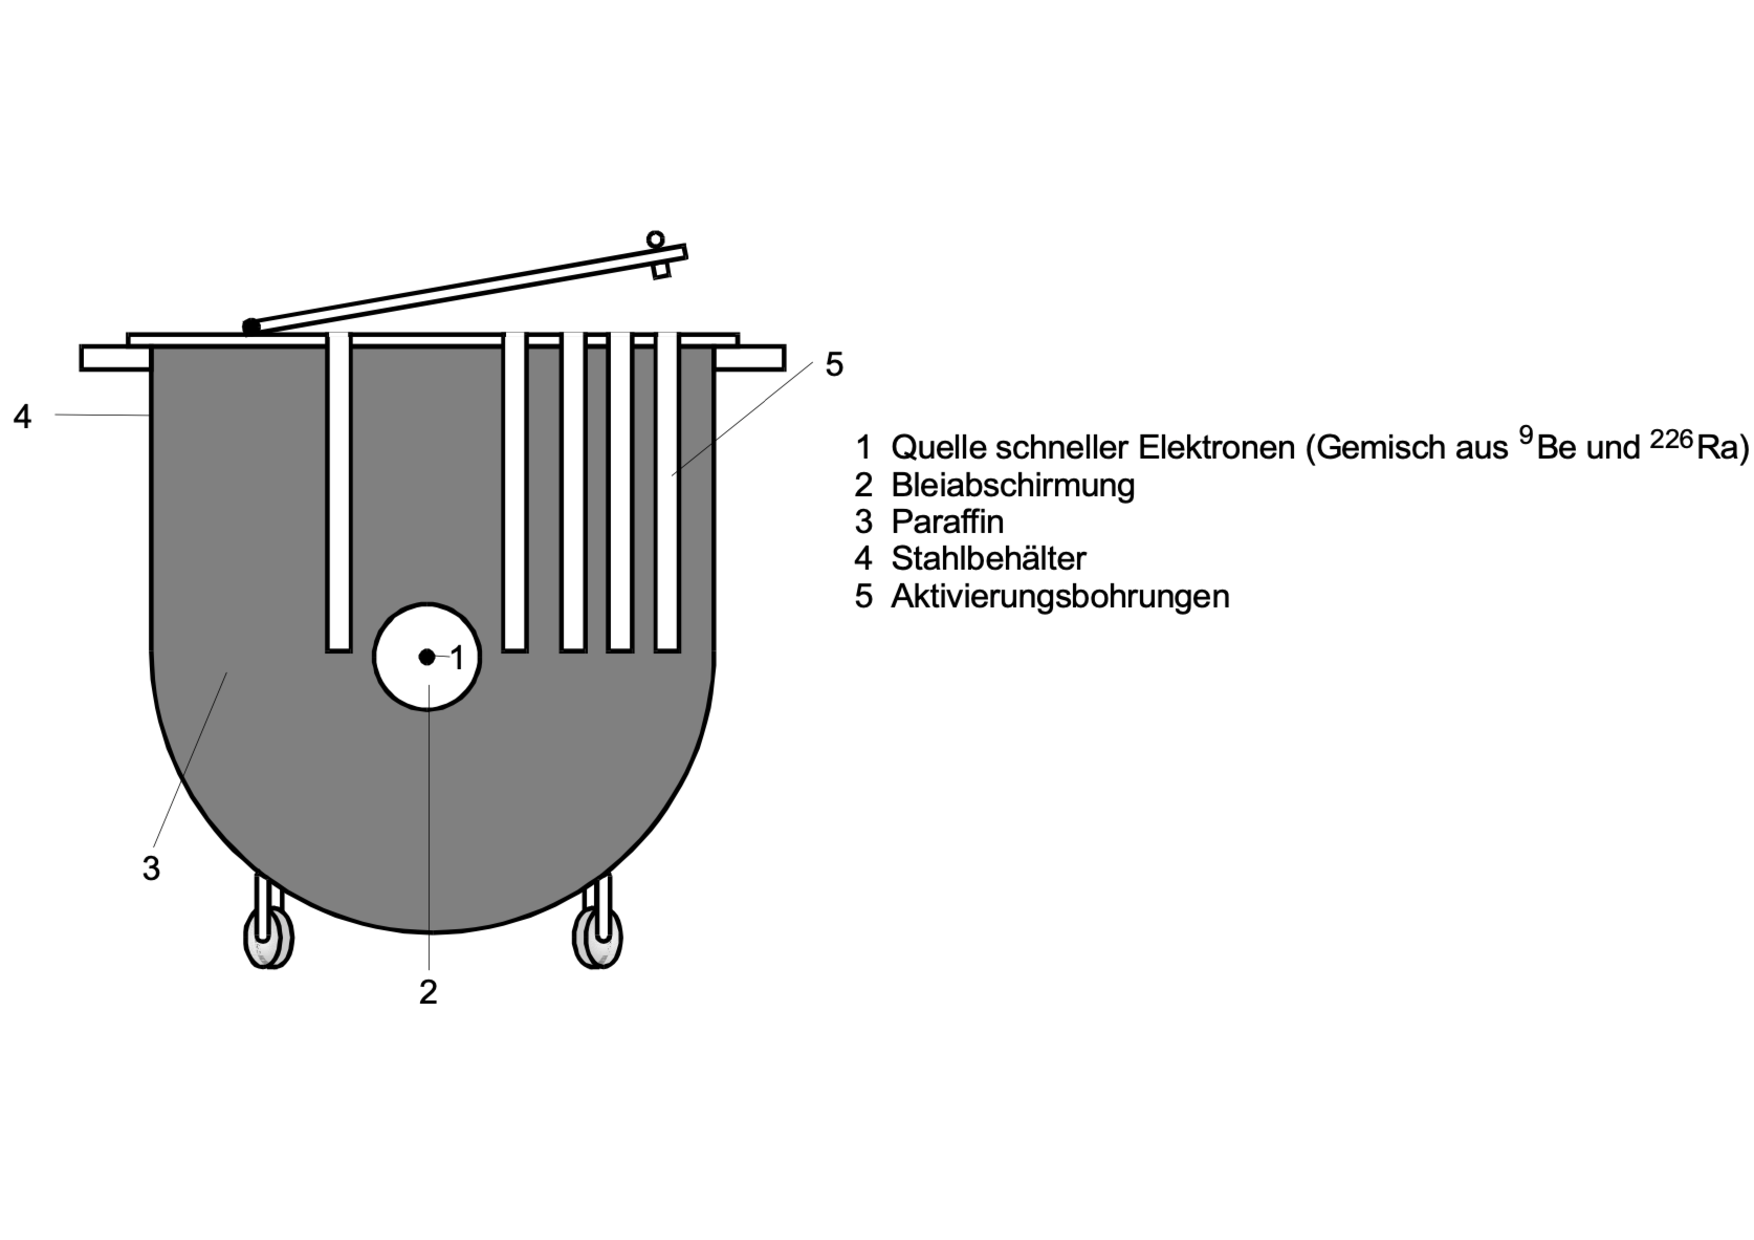
\includegraphics[height=5cm]{neutronenquelle.pdf}
               \caption{Querschnitt durch die hier verwendete Neutronenquelle (Quelle: \cite{V702}).}
               \label{fig:nq}
\end{figure}

\newpage
\subsection{Zerfall instabiler Isotope}

\noindent
Um den Zerfall instabiler Isotope zu untersuchen, werden zylindrische Proben, die diese Nuklide enthalten,
in die Aktivierungsschächte der Neutronenquelle aus Abbildung (\ref{fig:nq}) gebracht.
Der Zerfall der Isotope, auf die sich in diesem Versuch bezogen wird, sind gegeben durch:

\begin{equation}
\ce{_{23}^51V + n -> _{23}^52V -> _{24}^{52}Cr + }\beta^- \ce{+ \bar{\symup{\nu}}_e}
\end{equation}

\begin{equation}
\ce{^{103}_{45}Rh + n}&
  \begin{cases}
  \overset{10\%}{\ce{->}} \ce{^{104i}_{45}Rh
  -> ^{104}_{45}Rh} + \gamma \ce{-> ^{104}_{46}Pd + \beta^{-} + \bar{\nu}_e} \\
  \overset{90\%}{\ce{->}} \ce{^{104}_{45}Rh -> ^{104}_{46}Pd + \beta^{-} + \bar{\nu}_e}
  \end{cases}.
  \label{eqn:rh}
\end{equation}

\noindent
Wie in Gleichung (\ref{eqn:rh}) beschrieben, laufen bei der Aktivierung von Rhodium zwei Zerfälle parallel mit unterschiedlichen Halbwertszeiten ab.

\noindent
Der radioaktive Zerfall kann allgemein durch exponentiellen Zerfall beschrieben werden.
Die Anzahl der zu einem Zeitpunkt t noch nicht Zerfallenen Kerne lässt sich ausdrücken durch

\begin{equation}
\text{N}(\text{t}) = \text{N}_0 e^{-\lambda \text{t}},
\label{eqn:n}
\end{equation}

\noindent
wobei $\text{N}_0$ die Anzahl der Kerne zum Zeitpunkt t=0 und $\lambda$ die Zerfallskonstante ist.
Die Halbwertszeit lässt sich durch einsetzen von N(T)=$\frac{1}{2} \text{N}_0$ in Gleichung (\ref{eqn:n}) bestimmen:

\begin{equation}
\text{T} = \frac{\text{ln}(2)}{\lambda}.
\label{eqn:T}
\end{equation}

\noindent
Da es nicht möglich ist, N(t) zuverlässig zu ermitteln, wird die Halbwertszeit durch einen anderen Ansatz ermittelt.
Hierzu wird eine Anzahl $\text{N}_{\Delta\text{t}}(\text{t})$ der in einem Intervall $\Delta\text{t}$ zerfallenen Kerne wie folgt definiert:

\begin{equation}
\text{N}_{\Delta\text{t}}(\text{t}) = \text{N}(\text{t}) - \text{N}(\text{t} + \Delta \text{t})
\label{eqn:nd}
\end{equation}

\noindent
Wird Gleichung (\ref{eqn:n}) in (\ref{eqn:nd}) eingesetzt, 
kann durch lineare Ausgleichsrechnung mit den Wertepaaren $\{ \text{ln}(\text{N}_{\Delta \text{t}}(\text{t}_\text{i})),\text{t}_\text{i}\}$
die Zerfallskonstante genauer ermittelt werden.
Dabei sollte das Zeitintervall $\Delta \text{t}$ passend gewählt und eventuell durch einen Vorversuch ermittelt werden.
